\subsection{EEV driver program: JSEISAN}
\index{JSEISAN} 

Software and manual by Bladimir Moreno 

JSEISAN is a JAVA application for providing a user-friendly graphical interface of some of the functions of the SEISAN earthquake analysis system. The program uses the functions implemented in SEISAN by executing external commands, which mean that most of the data processing is performed with the SEISAN software. JSEISAN is mainly a tool for formatting the input data and display the results. The program was developed with Visual Cafe 4 Standard Edition. The software operates in Unix and Windows environments. 

Using JSEISAN 

The program is started by giving command jseisan and the window 
(Figure \ref{fig:jseisan}) below will appear. 

\begin{figure}
\htmlimage{scale=2.0}
\centerline{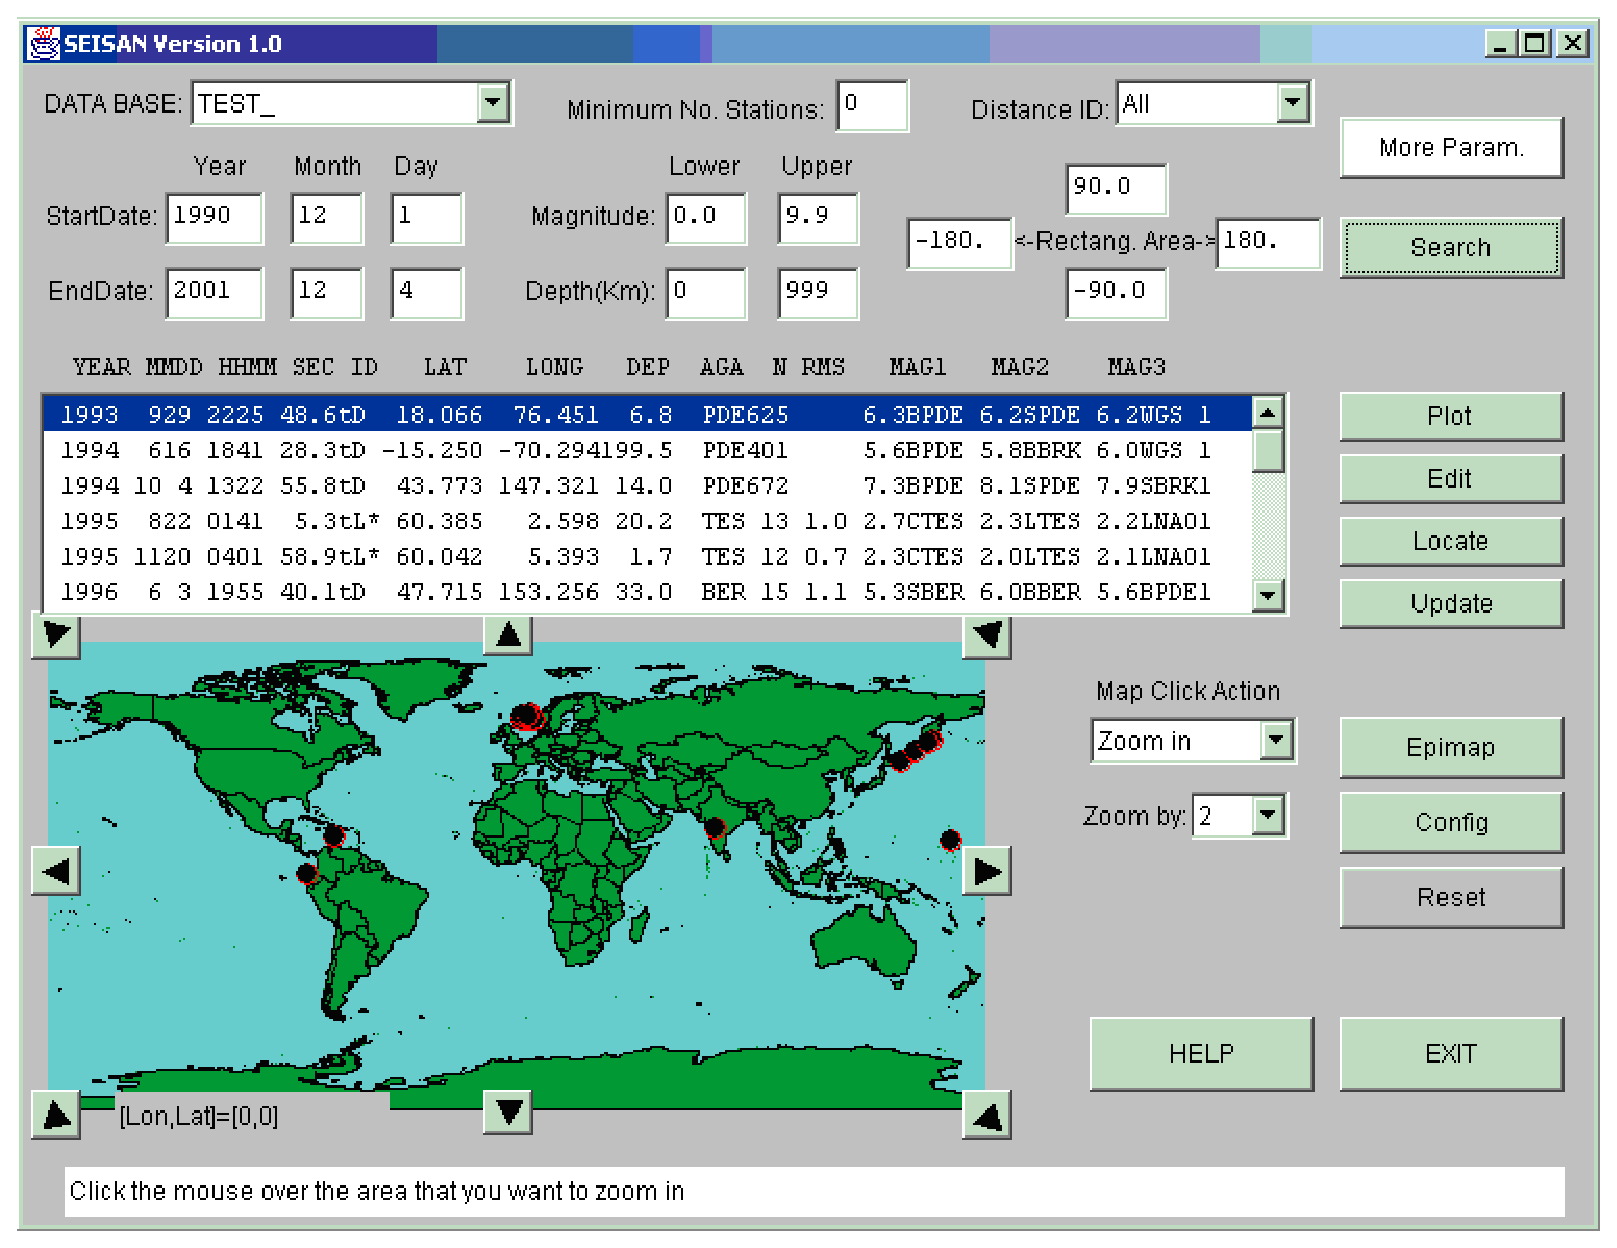
\includegraphics[width=0.9\linewidth]{fig/fig6}}
\caption{Main window of JSEISAN.}
\label{fig:jseisan}
\end{figure}

The user interaction with JSEISAN can be classified as: (1) Searching for earthquakes and (2) working with a particular earthquake. It is assume that a standard SEISAN data base is available with S-files and CAT files in the CAT directories (see SEISAN manual). The interface has a main window where the user can search earthquakes ($<$Search$>$ button) set up by a range of values 
(Figure \ref{fig:jseisan-Dialog-window}). 
As a result of the searching process, an earthquake list is shown on the screen and a set of functions is offered. In addition, the epicenters of the earthquake list are plotted on the map. Because there is a direct link between the map and the list, the selected earthquake is highlight on both the map and the list when the user is navigating either through the list or through the map (\textbf{see Interactive mapping tool}). 

Configuring JSEISAN 

JSEISAN \index{JSEISAN, configure}has several configuration variables to be set up by the user. In order to configure the variables, you have to click the button $<$Config$>$ (Figure \ref{fig:jseisan}). The configuration parameters are stored in the file \texttt{SEISAN.DEF}. \index{SEISAN.DEF}The editing process of this file is performed through the JAVA program \texttt{SEISCONF.class} (see SEISCONF). A complete description of the configuration parameters is given in at the end of this section. 



\textbf{Selecting the database to work with}

The desired SEISAN database is selected from the combo-box labeled as ``DATA BASE'' located in the left upper part of the main window (Figure \ref{fig:jseisan}). The last item in the combo-box corresponds to a SEISAN CAT file labeled as ``USER FILE''. When this item is selected, the user can load a file, for example \texttt{collect.out}, to work with. 

\textbf{Searching}

\index{Searching in the data base}
There are two windows for setting the parameters used in the searching process: (1) A main window, which contains the most common parameters (Figure \ref{fig:jseisan}) and 
(2) 
A second window (Figure \ref{fig:jseisan-Dialog-window}) which contain the rest. This second window is opened by clicking the button $<$More Param.$>$. In order to perform the search you have to: 

\begin{enumerate}
\item Set up the parameters (period of time, magnitude range, geographic area, etc.) needed in the searching process. 
\item Click the button $<$More Param.$>$ for refining the searching process (if needed). A dialog-box (Figure \ref{fig:jseisan-Dialog-window}) for setting the additional parameters is shown. 
\item Press the $<$Search$>$ button. 
\end{enumerate}


\begin{figure}
\htmlimage{scale=2.0}
\centerline{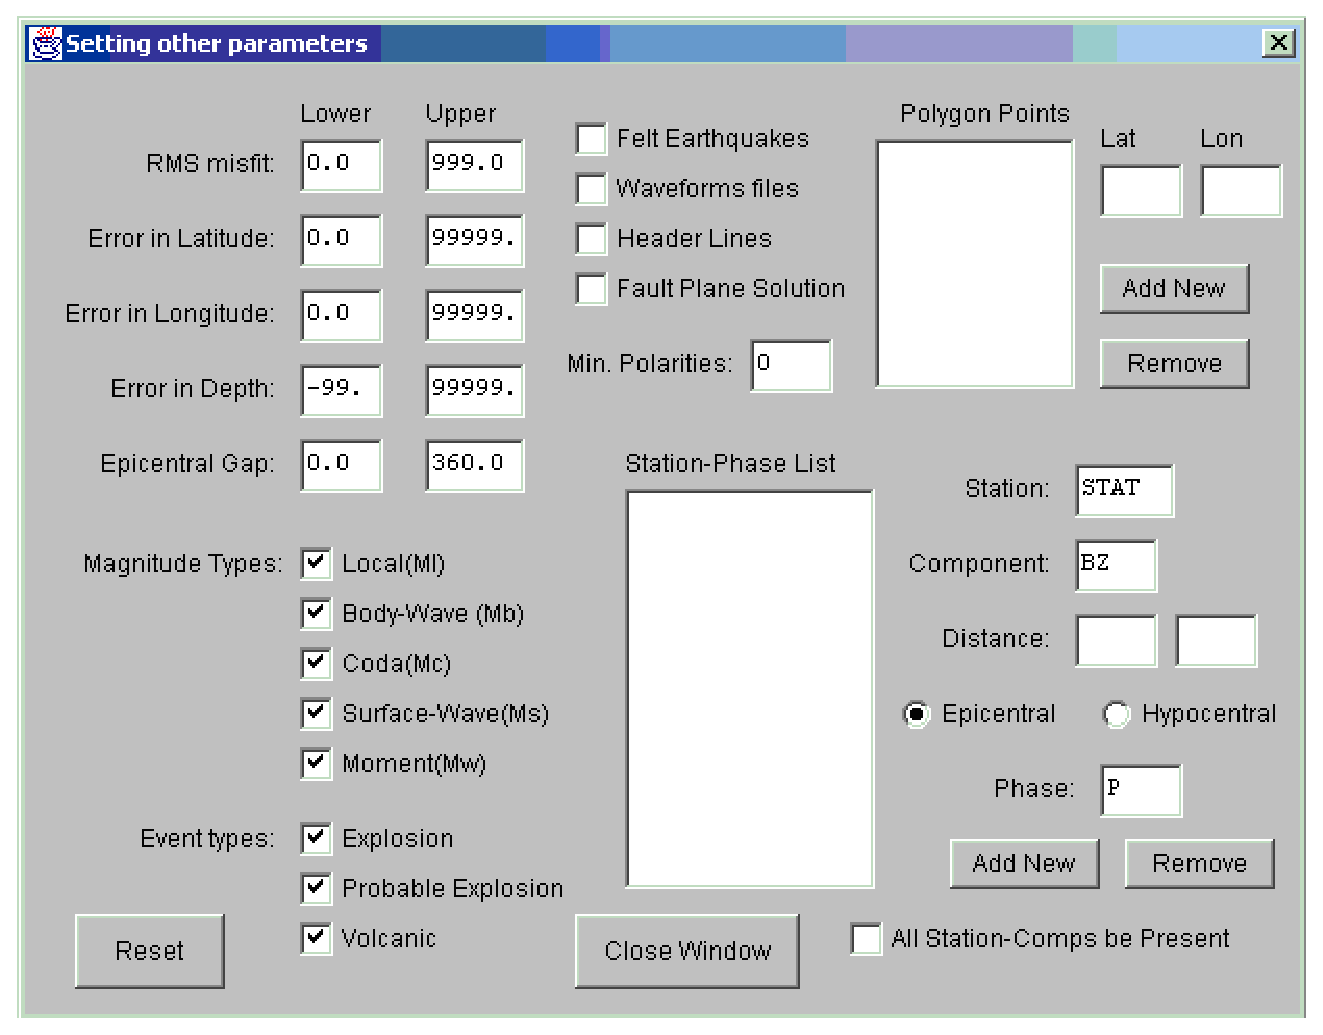
\includegraphics[width=0.9\linewidth]{fig/fig7}}
\caption{Dialog-window for setting other parameters used during search.}
\label{fig:jseisan-Dialog-window}
\end{figure}

Interactive Mapping Tool 

Figure \ref{fig:jseisan} shows a map with the locations of the earthquakes obtained during the searching process. The map has an equidistant cylindrical projection, which means that one unit of longitude has the same distance to one unit of latitude. This map can be used as interactive mapping tool. For this purpose, 4 options are included in the combo-box labeled as ``Map Click Action'' (Figure \ref{fig:jseisan}). The options are ``Select'', ``Zoom in'', ``Zoom out'' and ``Polygon''. The function of each radio-button is as follows: \index{MAP} 

``Select'': When it is active, the user can click over the circle identifying the location of the earthquake. The associated earthquake in the list will be highlighted. 

``Zoom in'': When it is active, the user can zoom in the map by a factor of 2,4,8,16 or 32. The zoom factor is selected from the combo-box labeled as ``Zoom by''. The clicked point on the map will be the center of the new map. \index{SELECT}\index{Zoom in map} 

``Zoom out'': Similar to ``Zoom in'' but with reverse effect. 

``Polygon'': When it is active, the user can define the points of a polygon by clicking on the map. The polygon is closed when a click over the starting point is made. Once the polygon is defined, the user can edit its points by using the refined search window, which is reach by clicking the $<$More Param.$>$ button. Epicenters inside the polygon can now be selected with the search function. \index{Polygon, select in} 

The zoomed map is taken either from Internet or locally. In the case of being retrieved locally, the images are taken from the directory specified by the configuration variable \textbf{IMGMAP\_PATH}. The images are saved in sub-directories according with the level of zoom. For example in case of 6 levels of zoom you will find the directories ZOOM0, ZOOM1, ZOOM2, ZOOM3, ZOOM4, ZOOM5 and ZOOM6. ZOOM0 only has one image, the whole world. ZOOM1 contain 9 images, the world is divided into 9 equal areas. ZOOM2 contain 81 images, the world is divided into 81 areas and the last 
6
level of zoom (ZOOM6) contains $9^{6}$ images. The image files are numbered as IMG\#.gif from left-up to right-down, like a matrix but using only one index. When the map is being retrieved from Internet there is no zooming limitation. You can go as deep as you want. The configuration variable \textbf{MAP\_SERVER} controls where to retrieve the image from. 

\textbf{Making an epicenter map from the earthquake list}

An epicenter map can be made through the SEISAN command ``EPIMAP''. The steps are:  \index{EPIMAP} 

\begin{enumerate}
\item Press the $<$Epimap$>$ button 
\item A new dialog-box for the configuration of the map is shown 
(Figure \ref{fig:jseisan-Dialog-box}), then click the  $<$Ok$>$ button. 
\end{enumerate}

\begin{figure}
\centerline{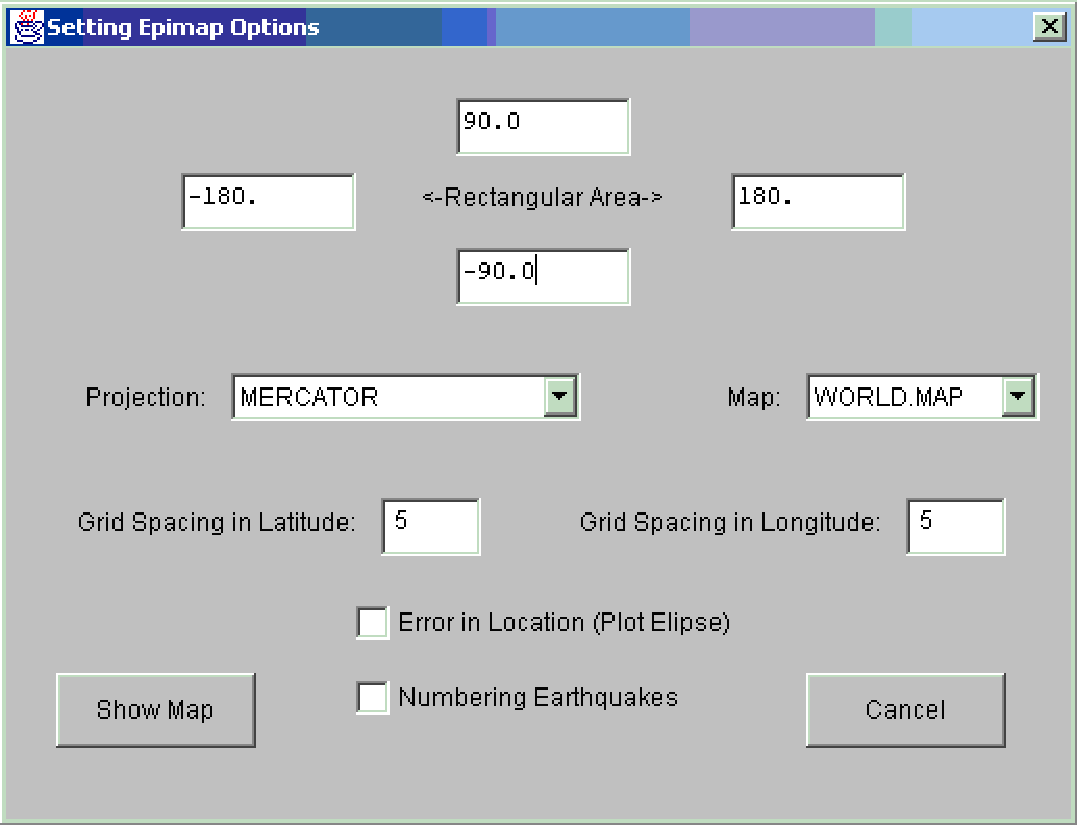
\includegraphics[width=0.9\linewidth]{fig/fig8}}
\caption{Dialog-box for setting the EPIMAP input data. Only the most common EPIMAP parameters are set.}
\label{fig:jseisan-Dialog-box}
\end{figure}

\textbf{Working with a particular earthquake}\newline
There are four available options for working with a particular earthquake of the list: (1): Plot waveforms, (2) Edit phases, (3) Locate and (4) Update. The associated buttons are located on the right side of the earthquake list (Figure \ref{fig:jseisan}). 

\textbf{Plotting and processing traces}\newline
Any number of channels, up to 75, can be plotted. In order to visualize a large number of channels, a page system is implemented, when more than 12 channels are selected. For practical reason, two operation modes are given in the plotting process: 
``multi-traces mode'' (Figure \ref{fig:jseisan-Multi-Trace-mode}) and ``single-trace mode'' 
(Figure \ref{fig:jseisan-Single-Trace-mode}). 
The distinction is made mainly for choosing which channels will be plotted together (multi-trace mode with select/unselect) and to navigate through the selected channels in more detail (single-trace mode). This is similar to MULPLT in SEISAN. In both operational modes, picking phases, zooming and filtering can be done. For ``multi-trace mode'', a set of additional options are available, e.g. save traces, which is applied to the plotted channels on the screen within a selected time window. 

\begin{figure}
\htmlimage{scale=2.0}
\centerline{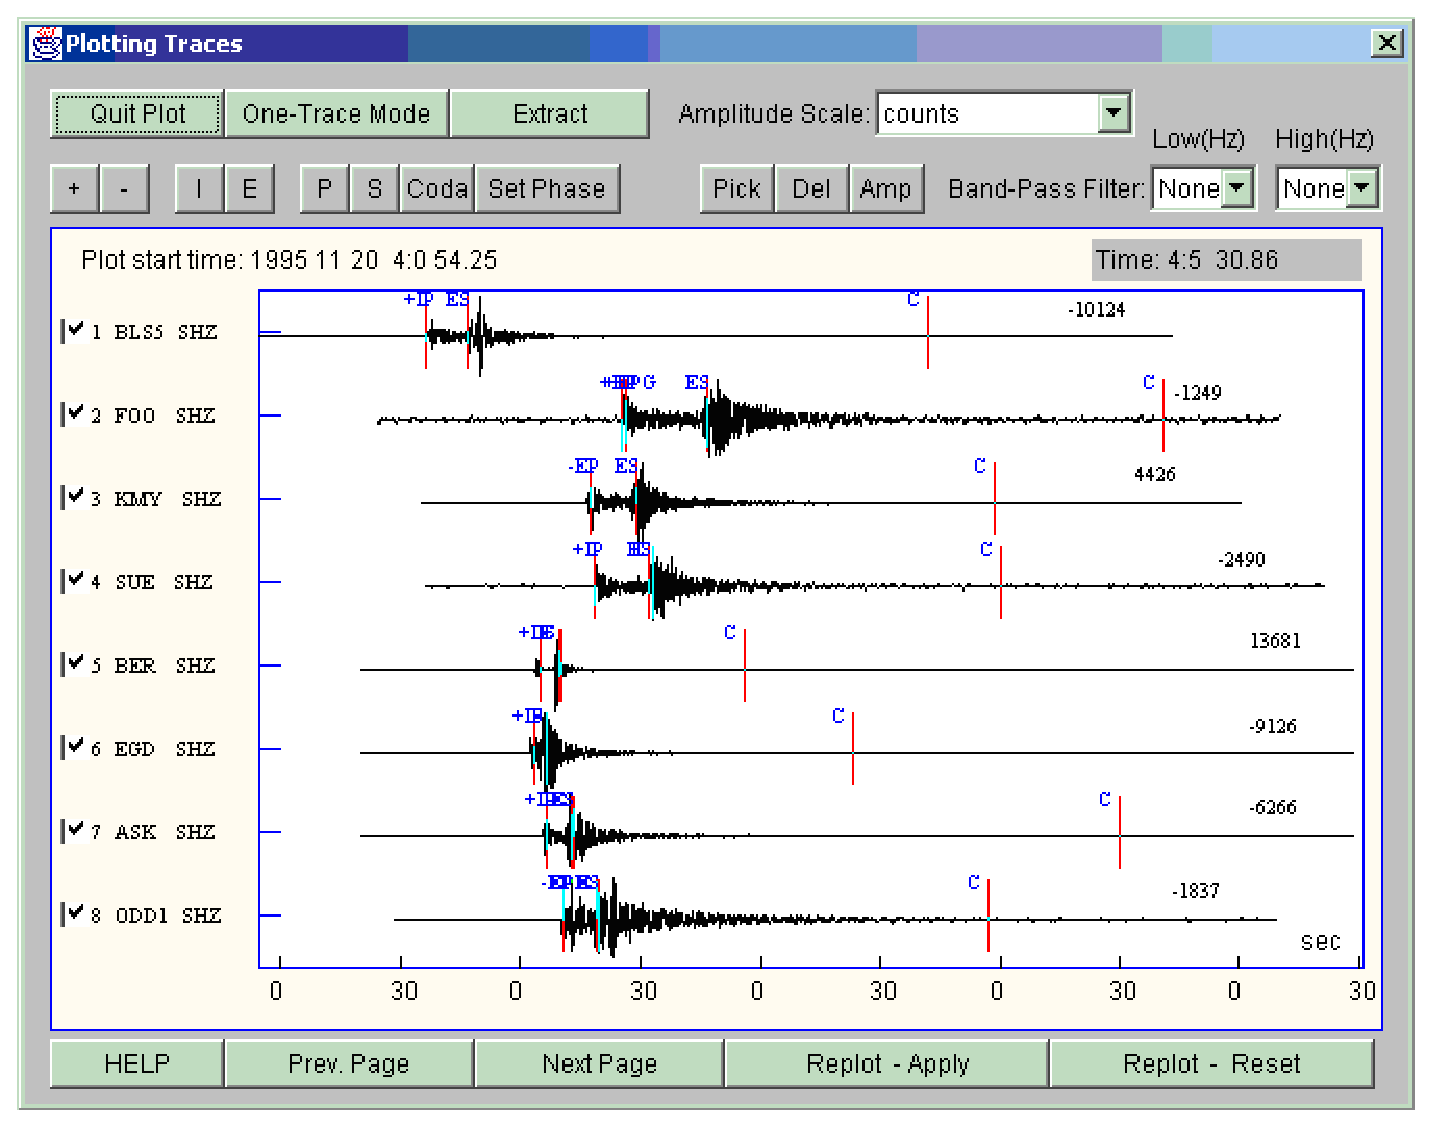
\includegraphics[width=0.9\linewidth]{fig/fig9}}
\caption{ Plotting window. Multi-Trace mode.}
\label{fig:jseisan-Multi-Trace-mode}
\end{figure}

\begin{figure}
\htmlimage{scale=2.0}
\centerline{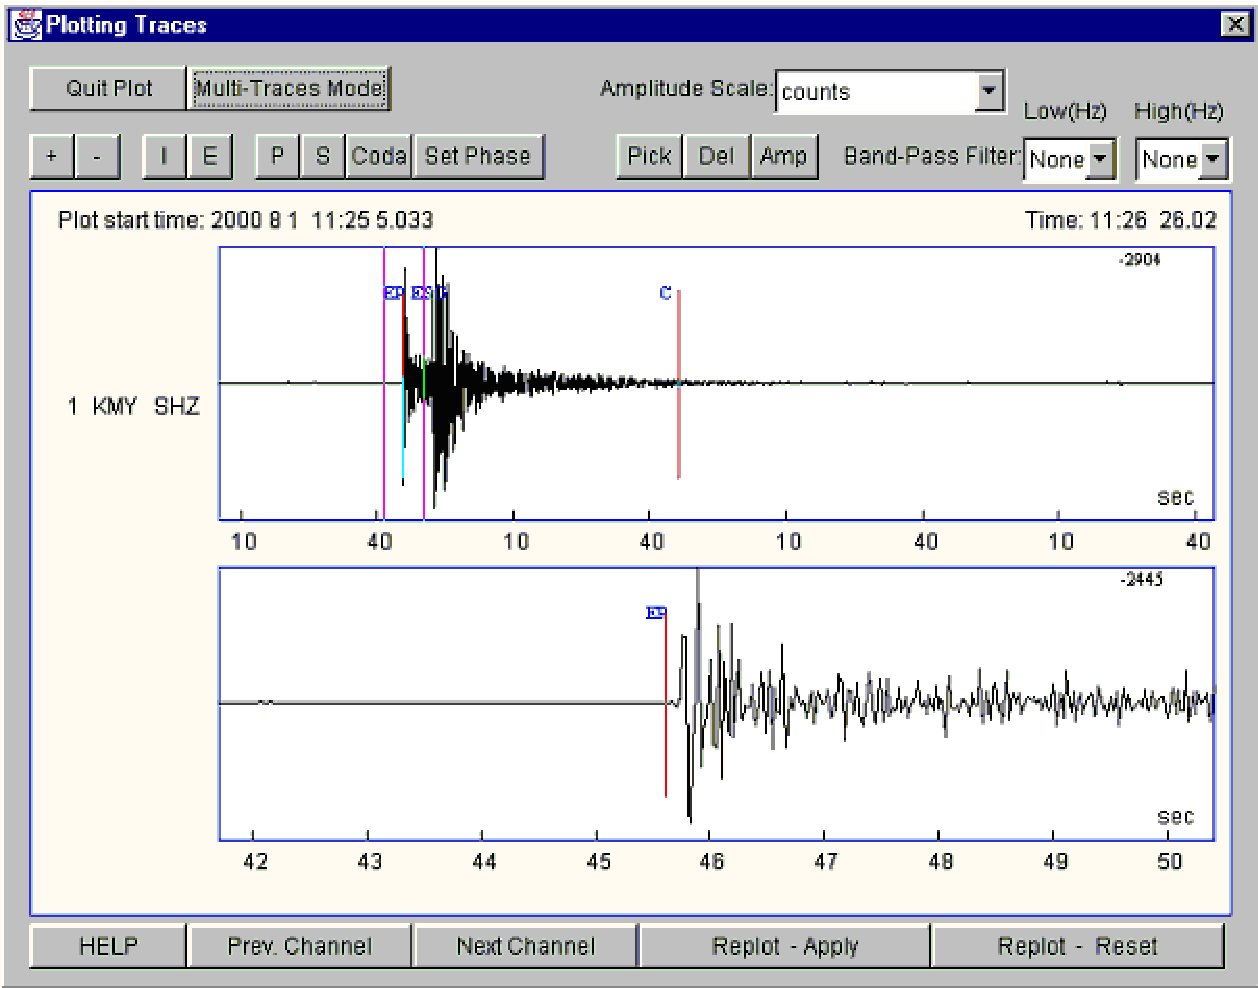
\includegraphics[width=0.9\linewidth]{fig/fig10}}
\caption{ Plotting window. Single-Trace mode.}
\label{fig:jseisan-Single-Trace-mode}
\end{figure}

The steps to plot a particular earthquake selected from the list are: 
\begin{enumerate}
\item Select a desired earthquake from the list by clicking the left button of the mouse on it (Figure \ref{fig:jseisan}). 
\item Press the $<$Plot$>$ button. 
\item A new dialog-box for the selection of the channels to be plotted is shown (Figure \ref{fig:jseisan-Selection-of-channels}), then click the $<$Plot$>$ button. 
\end{enumerate}

\begin{figure}
\htmlimage{scale=2.0}
\centerline{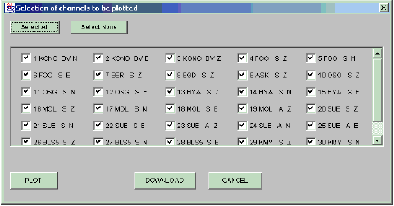
\includegraphics[width=0.9\linewidth]{fig/fig11}}
\caption{Selection of channels.}
\label{fig:jseisan-Selection-of-channels}
\end{figure}

Filtering one/several channels 
\begin{enumerate}
\item Select the low corner frequency of the Band-Pass filter (select ``none'' if a High-Pass filter is desired) from the combo-box labeled as ``Band-Pass filter'' 
(Figure \ref{fig:jseisan-Multi-Trace-mode}).  
\item Select the high corner frequency of the Band-Pass filter (select ``none'' if  a Low-Pass filter is desired). 
\item Make a zoom over the traces (\textbf{see Zooming section}) or click the button $<$Replot - Apply$>$\index{Zoom in JSEISAN} 
\end{enumerate}

\textbf{Instrument corrections}\newline
Converting the amplitude of one/several\index{Response removal} traces into ground velocity, displacement or acceleration and simulating Wood-And., Mb and Ms amplitude. 

\begin{enumerate}
\item Select the desire amplitude from the combo-box labeled  ``Amplitude Scale'' 
(Figure \ref{fig:jseisan-Multi-Trace-mode}). 
\item Make a zoom over the traces (\textbf{see Zooming section}) or click the button $<$Replot - Apply$>$ 
\end{enumerate}

\textbf{Picking and removing phases}\newline
\index{Phase picking} 
\begin{enumerate}
\item
 Press the $<$+$>$/$<$-$>$ button (Figure \ref{fig:jseisan-Multi-Trace-mode}) 
in order to select/unselect the polarity (Compression/ Dilatation) of the first impulse (if needed) 
\item Press the $<$I$>$/$<$E$>$ button in order to select/unselect the shape (Impulsive/Emergent ) of the first impulse (if needed) 
\item Press the button identifying the phase to be picked/removed ($<$P$>$/$<$S$>$,\dots ) 
\item Press the $<$Pick$>$/$<$Del$>$ button to active the picking/deleting process 
\item Move the mouse pointer to the position of the first impulse 
\item Click the left button 
\end{enumerate}


* The previous buttons will be kept active. Furthermore you can pick the selected phase for the rest of the channels without going through the first 4 steps. 

Reading amplitude \newline
\begin{enumerate}
\item
 Press the $<$Amp$>$ button (Figure \ref{fig:jseisan-Multi-Trace-mode}) 
to active the reading process 
\item Move the mouse pointer to the position of one extreme (upper or lower) of the signal    
\item Click the left button (a horizontal line will be drawn) 
\item Move the mouse pointer to the position of the opposite extreme of the signal one half period away.  
\item Click the left button 
\end{enumerate}

* The $<$Amp$>$ button will be kept active. Furthermore you can continue reading amplitudes for the rest of the channels without going through the first step. 

Zooming \newline
\begin{enumerate}
\item
 Move the mouse pointer to the initial time of the zooming window (the time is shown above the right-upper-corner when you move the mouse) 
\item Click the left button 
\item Move the mouse pointer to the final time of the zooming window 
\item Click the left button 
\end{enumerate}


Extracting traces from a time window \newline
You can extract either raw or processed traces from the plotting window 
(Figure \ref{fig:jseisan-Multi-Trace-mode}). The steps are: 

\begin{enumerate}
\item
 Select/unselect (see ``Other options'' section) the channels to be downloaded  
\item Make any desire processing (zoom, filter, etc.) if you want to save  processed traces or a data selection of the original traces. 
\item Press the $<$DownLoad$>$ button. \index{Extract data in JSEISAN} 
\end{enumerate}


The data will now be stored in your working directory in SEISAN format in a file with name specified by the user. Since an integer format is used, processed data with amplitudes less than 1 will have amplitude values 0. 

Other options 

Switching between ``single'' and ``multi'' traces mode 

\begin{enumerate}
\item
Press the $<$single-trace mode$>$/$<$multi-traces mode$>$ button 
(Figure \ref{fig:jseisan-Multi-Trace-mode} and Figure \ref{fig:jseisan-Single-Trace-mode}). 
\end{enumerate}

Show/hide channels to be plotter together on the screen 

\begin{enumerate}
\item
 Press the $<$Replot - Reset$>$ button (Figure \ref{fig:jseisan-Multi-Trace-mode}) 
\item
 Click the left button of the mouse over the check-box identifying each channel in order to select/unselect the channel 
\item
 Press the $<$Replot - Apply$>$ button 
\end{enumerate}


Navigating through individual channels \newline
\begin{enumerate}
\item
 Go to the ``single-trace'' mode (Figure \ref{fig:jseisan-Single-Trace-mode}). 
\item
 Press the $<$Next Channel$>$ button to go forward or $<$Previous Channel$>$ to go backward 
\end{enumerate}


Navigating through pages of channels (12 channels as maximum on one page) \newline
\begin{enumerate}
\item
 Go to the ``multi-trace'' mode (Figure \ref{fig:jseisan-Multi-Trace-mode}) 
\item
 Press the $<$Next Page$>$ button to go forward or $<$Previous Page$>$ to go backward 
\end{enumerate}


Editing S-files\newline
The editing window (Figure 
\ref{fig:editing-window}
) has 3 buttons for closing the window. When you click the button $<$Save \& Exit$>$ the S-file is physically modified on the hard disk. The $<$close$>$ button keeps the changes in memory until another earthquake is selected on the list. So, you can still perform full processing without making any real change in the S-file. The steps to edit the S-file are: 

\begin{enumerate}
\item
 Select a desired earthquake from the list clicking the left button of the 
mouse on it (Figure \ref{fig:jseisan})
\item
 Click the $<$Edit$>$ button 
\item
 An editing window with the information is shown (Figure \ref{fig:editing-window}).
\end{enumerate}

\begin{figure}
\htmlimage{scale=2.0}
\centerline{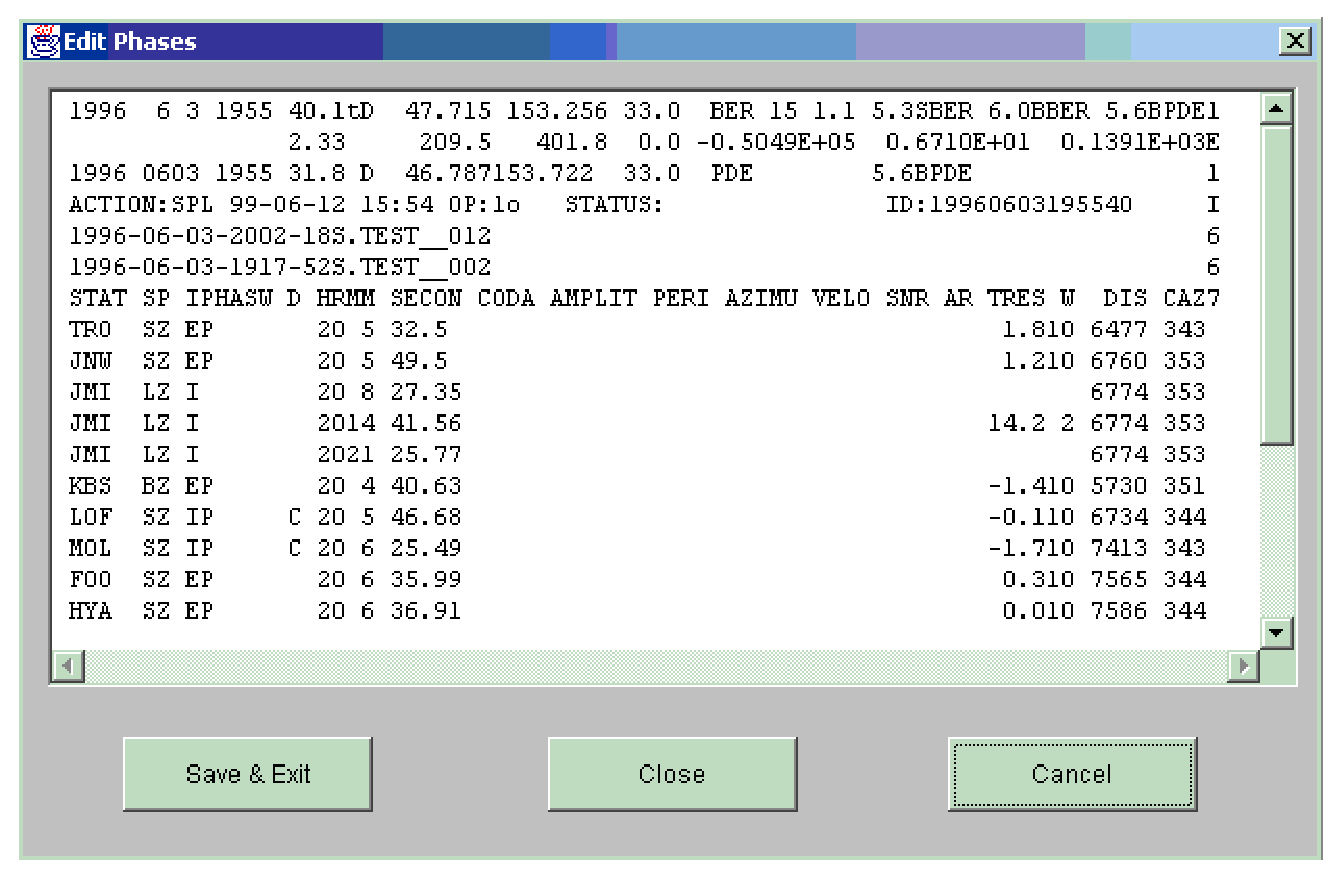
\includegraphics[width=0.9\linewidth]{fig/fig12}}
\caption{Editing window.}
\label{fig:editing-window}
\end{figure}

Note that this editing function do not yet, as in SEISAN EEV, check the file for correct editing. 

Determining hypocenter and magnitude \newline
\begin{enumerate}
\item
 Select a desired earthquake from the list clicking the left button of the mouse on it 
\item
 Press the $<$Locate$>$ button 
\item
 A new window with the results is shown (Figure \ref{fig:hypocenter-determination}) 
\end{enumerate}

\begin{figure}
\htmlimage{scale=2.0}
\centerline{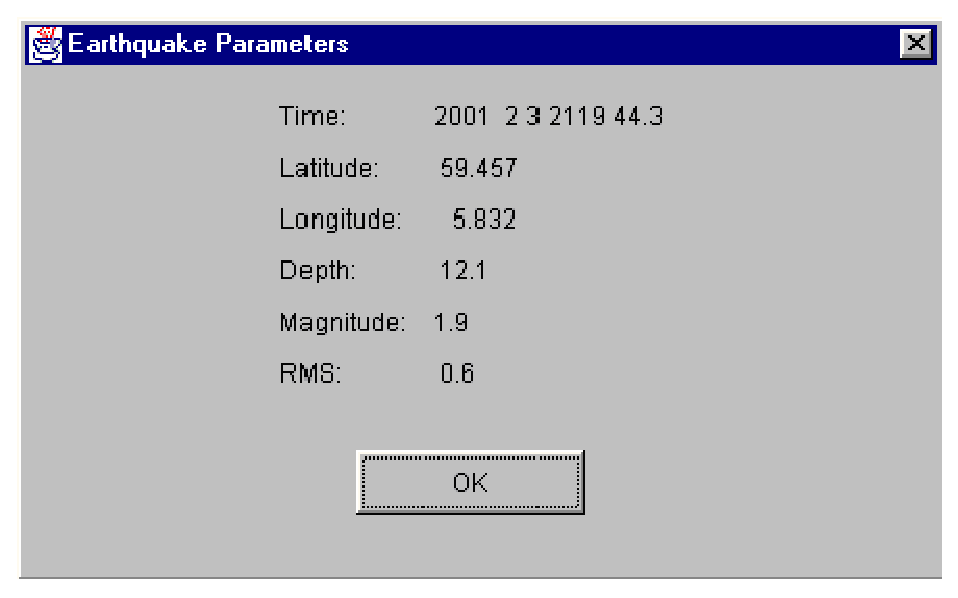
\includegraphics[width=0.9\linewidth]{fig/fig13}}
\caption{Results of the hypocenter determination.}
\label{fig:hypocenter-determination}
\end{figure}

The usual SEISAN files print.out and hyp.out are generated (see section 6.1.1).


Updating the earthquake in the database 

\begin{enumerate}
\item
Select a desire earthquake from the list by clicking the left button of the mouse. 
\item
Press the $<$Update$>$ button (Figure \ref{fig:jseisan}) 
\end{enumerate}

Note: This updates the S-file, but the original CAT file in the database is NOT updated. In order to do so, an update outside JSEISAN must be done (see SEISAN manual). 

Help Function\newline
\index{Help in SEISAN}
The help system implementation is based on PDF files. When the user clicks the $<$HELP$>$ button, a list of PDF files is shown 
(Figure \ref{fig:list-pdf-files}).
The list is stored in the file ``helpmenu.inp'', which is found in the DAT directory. You can edit this file for adding new PDF files to the help system 


\begin{figure}
\htmlimage{scale=2.0}
\centerline{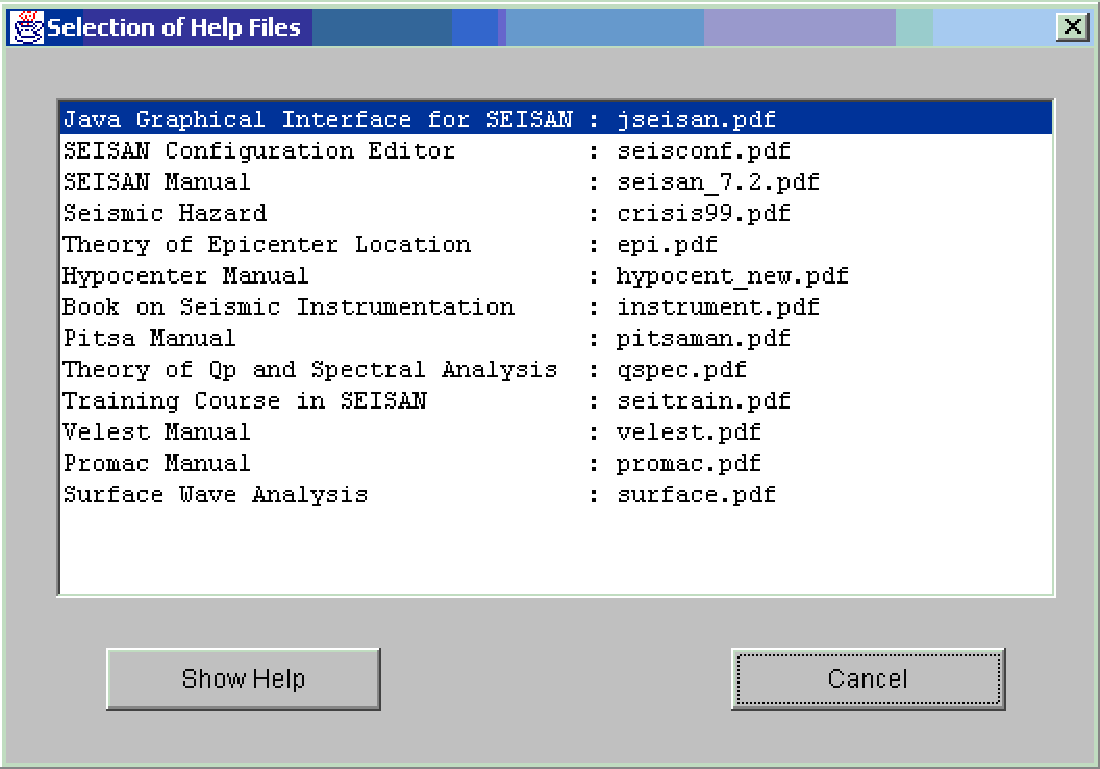
\includegraphics[width=0.9\linewidth]{fig/fig14}}
\caption{Example list of PDF files used for the help system, normally in DAT.}
\label{fig:list-pdf-files}
\end{figure}

\textbf{Configuration parameters in JSEISAN}

\index{SEISAN.DEF}\index{JSEISAN, configuration parameters}The following parameters used by JSEISAN are stored in the configuration file \texttt{SEISAN.DEF}. They can be edited through the program SEISCONF. Most of them are defined to be used only with JSEISAN, but some are already defined in the SEISAN configuration file: \texttt{SEISAN.DEF} ( EPIMAP\_PROJECTION and EPIMAP\_MAP\_FILE) 

\noindent
\textbf{OUTPUT\_DIR}: Output Directory for SEISAN commands results. Default ``./'' \newline
\textbf{EPIMAP\_MAP\_FILE}: Name of the map file for EPIMAP command \newline
\textbf{EPIMAP\_PROJECTION}: Number of the projection for EPIMAP command (see SEISAN Manual) \newline
\textbf{INIT\_IMGMAP\_FILE}: File name of the initial map represented as image. Default ``/seismo/DAT/IMGWORLD.gif''\newline
\textbf{MAP\_SERVER}: Type of map retrieved from Internet or locally; 0: Static local image (country boundaries), 1: Static remote image (country boundaries), 2,3,4,5: Dynamic Remote image (2:country boundaries, 3:Relief from GTOPO30 only land, 4:Two minute shaded relief, 5: Combine 3 and 4). Default 0. \newline
\textbf{IMGMAP\_PATH}: PATH for the static local maps (images) stored in the local hard disk used for zooming. Default ``/seismo/DAT/IMGMAP'' \newline
\textbf{INIT\_MAP\_LOWER\_LATITUDE}: Lower latitude of the initial map. Default -90.0 \newline
\textbf{INIT\_MAP\_UPPER\_LATITUDE}: Upper latitude of the initial map. Default 90.0 \newline
\textbf{INIT\_MAP\_LEFT\_LONGITUDE}: Lower longitude of the initial map. Default -180.0 \newline
\textbf{INIT\_MAP\_RIGHT\_LONGITUDE}: Upper longitude of the initial map. Default 180.0 \newline
\textbf{ACROBAT\_READER}: Path for the Adobe Acrobat Reader (needed for the help files). Default ``/prog/acroread'' for Unix. \newline
\textbf{INTERNET\_BROWSER}: Location and place of browser \newline
\textbf{HELP\_DIR}: Directory of help files, usually INF 

